\subsubsection{Giới thiệu}
Kiến trúc mạng thần kinh căn bản được thiết kế để nhận các điểm dữ liệu đầu vào có số chiều cố định, và thứ tự các điểm này không quan trọng. Tuy nhiên trong thực tế có nhiều loại dữ liệu có số chiều không cố định, hay có những dữ liệu mà thứ tự của nó quan trọng. Ví dụ dữ liệu là chuỗi các giá trị thực (\textit{real-valued}) như chuỗi thời gian (\textit{time-series}), hay dữ liệu là chuỗi các ký hiệu có thứ tự (\textit{symbolic}) như văn bản, dữ liệu sinh học. Những dữ liệu này mang đặc tính thứ tự \cite{Aggarwal2023}:
\begin{itemize}
    \item Trong chuỗi thời gian, các điểm dữ liệu được sắp xếp có quy luật. Nếu ta hoán đổi thứ tự các điểm sẽ làm mất đi tín hiệu trong chuỗi thời gian. Ngoài ra, giá trị tại thời điểm $t$ của chuỗi thời gian có mối liên quan chặt chẽ đến các giá trị trong cửa sổ (\textit{window}) trước đó.
    \item Khi ta thêm/bớt/đảo thứ tự một vài từ trong câu thì độ dài dữ liệu, ngữ nghĩa của câu có thể bị thay đổi hoặc không.
    \item Dữ liệu sinh học luôn tồn tại dưới dạng chuỗi, trong đó mỗi điểm dữ liệu là một axit amin, hoặc chi tiết hơn thì các điểm dữ liệu biểu thị cho một nuclêôtit.
\end{itemize}
\begin{figure}[htb]
    \centering
    \begin{subfigure}[t]{0.33\textwidth}
        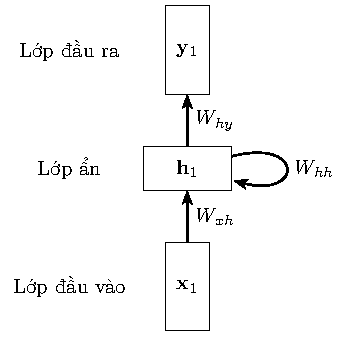
\includegraphics[width=\textwidth]{tikz_image/rnn_loop_architecture.pdf}
        \caption{Kiến trúc mạng hồi quy}
        \label{figure:rnn-loop-architecture}
    \end{subfigure}
    \begin{subfigure}[t]{0.66\textwidth}
        \centering
        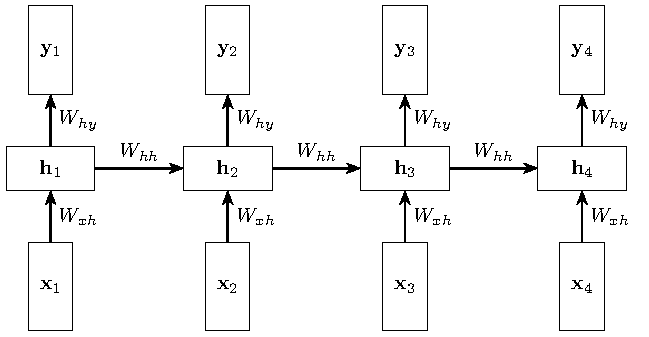
\includegraphics[width=\textwidth]{tikz_image/rnn_layer_architecture.pdf}
        \caption{Kiến trúc mạng hồi quy khi khai triển thành các lớp thời gian}
        \label{figure:rnn-layer-architecture}
    \end{subfigure}
    \caption{Mạng hồi quy \cite{Aggarwal2023}}
\end{figure}
\begin{figure}[htb]
    \centering
    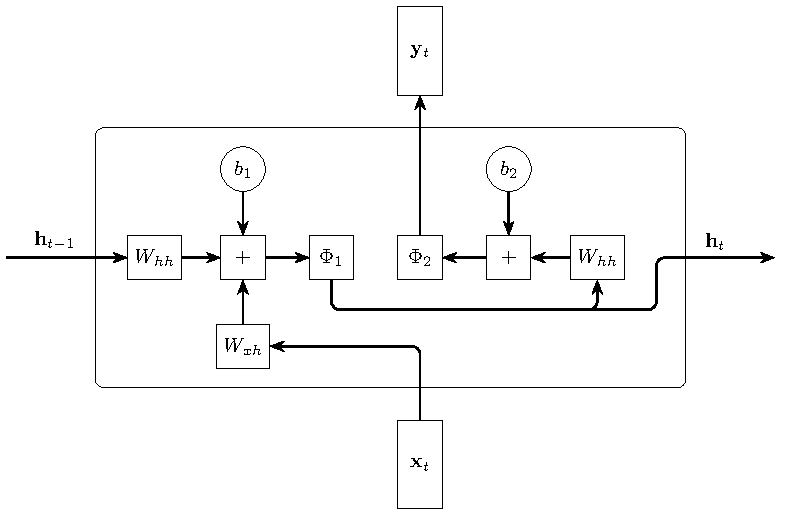
\includegraphics[width=0.7\textwidth]{tikz_image/rnn_hidden_layer_architecture.pdf}
    \caption{Kiến trúc của lớp ẩn trong mạng hồi quy}
    \label{figure:rnn-hidden-layer-architecture}
\end{figure}

Khi ta dùng dữ liệu ngắn hơn mạng thần kinh yêu cầu ở lớp đầu vào, ta phải thêm các điểm vô nghĩa vào; hoặc khi ta dùng dữ liệu có độ dài dài hơn, thì ta phải cắt bớt dữ liệu đi; hoặc khi ta dùng dữ liệu có tính tuần tự thì mạng thần kinh không thể xử lý tốt vì nó không quan tâm đến thứ tự các điểm nó được học. Để khắc phục điều này, người ta đã tạo ra một cấu trúc khác cho mạng thần kinh nhân tạo, đó là mạng thần kinh hồi quy (\textit{recurrent neural network - RNN})

Mạng thần kinh hồi quy là các mạng thần kinh nhân tạo kết nối với nhau để tạo thành đồ thị có hướng dọc theo một trình tự thời gian. Ý tưởng căn bản khi tạo ra mạng thần kinh hồi quy là xem mạng như một vòng lặp, các vòng lặp liên tiếp nhau cho phép mạng sử dụng thông tin từ các dữ liệu trước đó, và ta có thể xem nó như một loại bộ nhớ. Mạng có thể tăng giảm số lượng thần kinh tuỳ ý, điều này cho phép mạng tiếp nhận dữ liệu với bất kỳ chiều dài nào nên nó có thể áp dụng cho các tác vụ như nhận dạng chữ viết tay hay nhận dạng tiếng nói, là những tác vụ có tính chất kết nối, không phân đoạn.

Mạng thần kinh hồi quy mô phỏng hoạt động của não bộ con người, cho phép máy tính có thể nhận diện các khuôn mẫu sẵn có để xử lí các vấn đề thông thường. Mạng được tạo thành từ nhiều lớp thời gian (\textit{temporal layer}) (hình \ref{figure:rnn-layer-architecture}) tiếp nối nhau và có những hoạt động tương tự như hoạt động của các nơron trong não người. Từ đó, mạng thần kinh hồi quy có thể dự đoán các dữ liệu chuỗi theo một cách mà mạng thần kinh thường không thể.

\subsubsection{Phân loại}
Kiến trúc của RNN có thể thay đổi dựa trên bài toán cần xử lí, bài toán có thể có có một hay nhiều input và ouput. Dưới đây là một số kiến trúc RNN \cite{webpage6}:
\begin{itemize}
    \item \textbf{Một-một (one-to-one)} Chỉ có một cặp input-output ở kiến trúc này. Kiến trúc này thường được sử dụng trong các mạng neuron truyền thống.
    \item \textbf{Một-nhiều (one-to-many)} Một input duy nhất trong kiến trúc one-to-many có thể tạo ra rất nhiều output khác nhau. Kiến trúc này thường được sử dụng cho quá trình sản xuất nhạc.
    \item \textbf{Nhiều-một (many-to-one)} Ở kiến trúc này, một output duy nhất được tạo ra bằng cách kết hợp nhiều input từ các mốc thời gian khác nhau. Kiến trúc này thường được sử dụng trong các bài toán phân tích và nhận dạng cảm xúc, nơi các nhãn được định nghĩa bởi các chuỗi từ.
    \item \textbf{Nhiều-nhiều (many-to-many)} Kiến trúc này sử dụng một chuỗi nhiều input để sinh ra một chuỗi nhiều output. Ví dụ điển hình cho kiến trúc này là các hệ thống dịch thuật ngôn ngữ.
\end{itemize}
\begin{table}[htb!]
    \centering
    \caption{Một số loại RNN \cite{webpage6}}
    \begin{tabularx}{\textwidth}{ L{1} c L{1} }
        \toprule
        \textbf{Loại RNN}         & \textbf{Hình minh hoạ}                                                                     & \textbf{Ứng dụng}           \\\midrule
        Một-một $T_x=T_y=1$       & 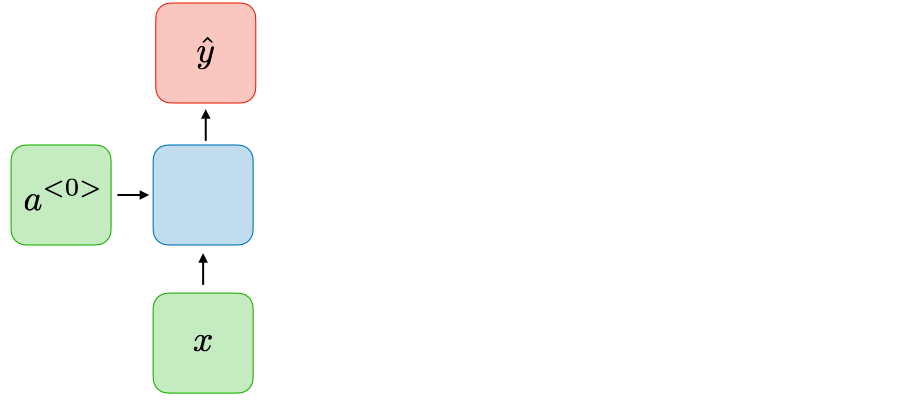
\includegraphics[width=0.47\textwidth, valign=c]{image/rnn-one-to-one-ltr.png}             & Mạng thần kinh truyền thống \\\midrule
        Một-nhiều $T_x=1,T_y>1$   & 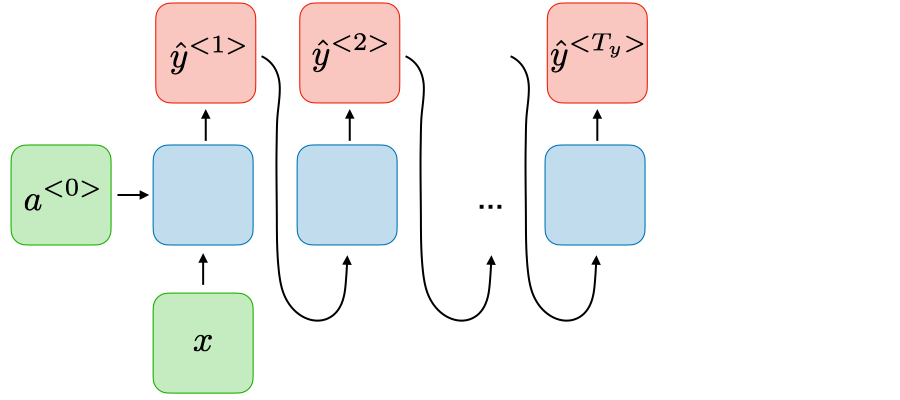
\includegraphics[width=0.47\textwidth, valign=c]{image/rnn-one-to-many-ltr.png}            & Sinh nhạc                   \\\midrule
        Nhiều-một $T_x>1,T_y=1$   & 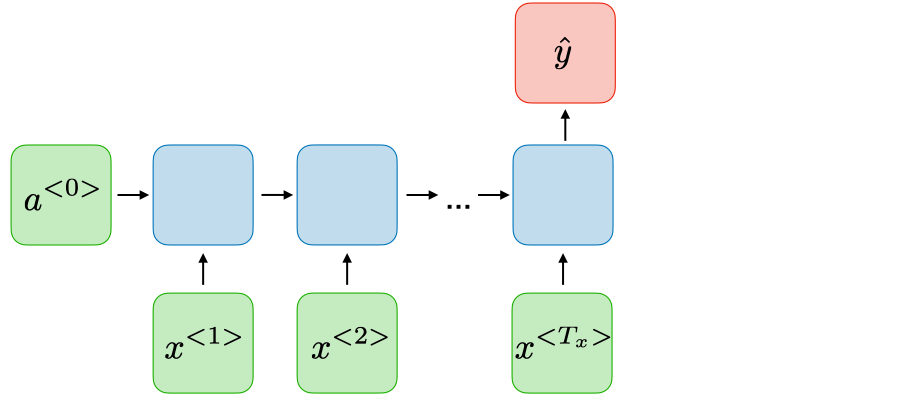
\includegraphics[width=0.47\textwidth, valign=c]{image/rnn-many-to-one-ltr.png}            & Phân loại cảm xúc, ý kiến   \\\midrule
        Nhiều-Nhiều $T_x=T_y$     & 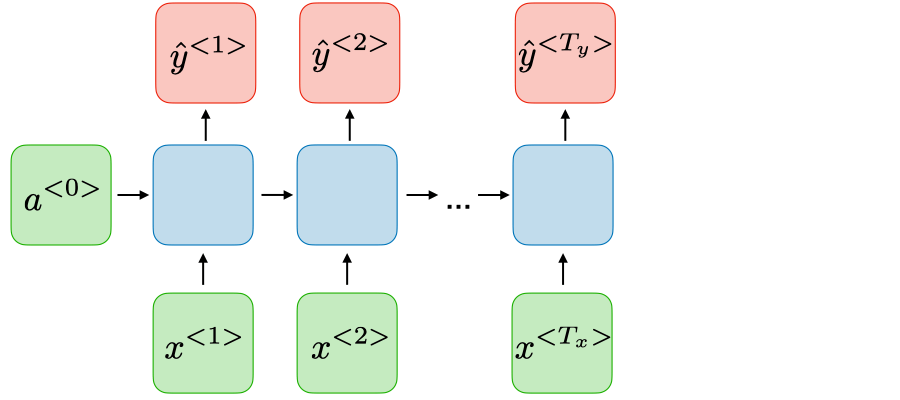
\includegraphics[width=0.47\textwidth, valign=c]{image/rnn-many-to-many-same-ltr.png}      & Nhận dạng tên của thực thể  \\\midrule
        Nhiều-nhiều $T_x\neq T_y$ & 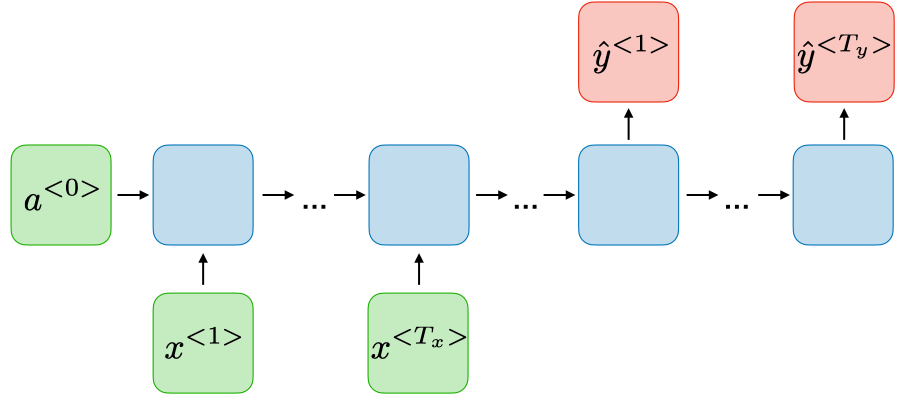
\includegraphics[width=0.47\textwidth, valign=c]{image/rnn-many-to-many-different-ltr.png} & Dịch                        \\
        \bottomrule
    \end{tabularx}
\end{table}

\subsubsection{Kiến trúc}
Dù mạng hồi quy được dùng trong hầu hết các lĩnh vực có tồn dữ liệu chuỗi, ứng dụng của nó trong lĩnh vực xử lí văn bản lại phổ biến và tự nhiên hơn cả. Dưới đây là hoạt động của mạng hồi quy trong ứng dụng dự đoán từ ngữ.
\begin{figure}[htb]
    \centering
    \begin{subfigure}[t]{0.33\textwidth}
        \centering
        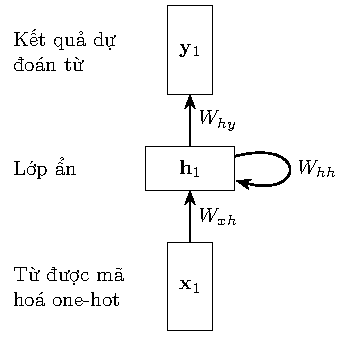
\includegraphics[width=\textwidth]{tikz_image/rnn_example_1a.pdf}
        \caption{Mạng hồi quy}
        \label{figure:rnn-example-a}
    \end{subfigure}
    \begin{subfigure}[t]{0.66\textwidth}
        \centering
        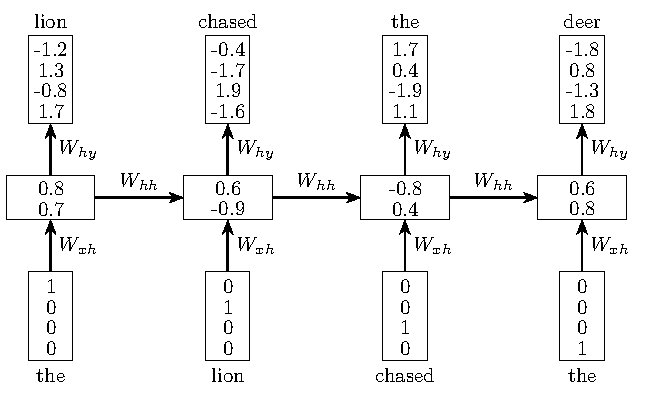
\includegraphics[width=\textwidth]{tikz_image/rnn_example_1b.pdf}
        \caption{Mạng hồi quy được trải thành lớp thời gian}
        \label{figure:rnn-example-b}
    \end{subfigure}
    \caption{Mạng hồi quy trong dự đoán từ \cite{Aggarwal2023}}
    \label{figure:rnn-example}
\end{figure}

Một mạng hồi quy được biểu diễn trên hình \ref{figure:rnn-example-a}. Điểm mấu chốt ở đây chính là vòng lặp tại chính giữa hình, thứ thay đổi trạng thái ẩn (\textit{hidden state}) của cả mạng sau mỗi từ trong chuỗi. Kiến trúc này trở nên rõ ràng hơn khi chúng ta “mở” vòng lặp đó ra trên một trục thời gian và biểu diễn giống như các mạng thần kinh nối tiếp nhau (hình \ref{figure:rnn-example-b}). Khi này chúng ta sẽ có những nút khác nhau đại diện cho lớp ẩn $\mathbf h_t$ trên mỗi điểm thời gian $t$. Dữ liệu đầu vào của nút thứ $n$ là từ thứ $n$. Cách trình bày này tương tự hình \ref{figure:rnn-example-a} nhưng dễ nắm bắt hơn do có sự tương đồng với các mạng thần kinh truyền thống. Ma trận $W$ trong các tầng khác nhau được sử dụng chung nhằm đảm bảo một hàm số duy nhất được sử dụng ở mỗi mốc thời gian. Dựa vào hình có thể thấy mỗi tầng đều có $W_{hh}$, $W_{hy}$, $W_{xh}$ giống nhau.

Trong bài toán dự đoán các từ tiếp theo khi đã biết các từ trước đó, ví dụ chúng ta có câu:\newline
\centerline{\textit{``The lion chased the deer''} \cite{Aggarwal2023}}
Khi từ ``The'' đi vào tầng đầu tiên, đầu ra sẽ là một vector chứa các xác suất của các từ bao gồm cả từ ``lion'', và khi từ ``lion'' là input của tầng tiếp theo, đầu ra vẫn là một vector như vậy. Đây là một phân loại của mô hình ngôn ngữ khi mà xác suất của một từ được ước lượng dựa trên lịch sử của các từ trước đó.

Với mốc thời gian $t$, vector đầu vào là $\mathbf x_t$, trạng thái ẩn là $\mathbf h_t$ và vector đầu ra  (trong ví dụ này là xác suất các từ có khả năng xuất hiện tại thời gian mốc thời gian $t+1$) là $\mathbf y_t$. Hai vector $\mathbf x_t$ và $\mathbf y_t$ sẽ có số chiều giống nhau là $d$, với $d$ là số từ khác nhau của câu (khi ta dùng mã hoá \textit{one-hot}). Trạng thái ẩn $\mathbf h$ tại $t$ được tính từ $\mathbf x_t$ và $\mathbf h_{t-1}$ thể hiện dưới dạng
\begin{align}
    \mathbf h_t & =W_{xh}\mathbf x_t+W_{hh}\mathbf h_{t-1}\label{equation:rnn-h} \\
    \mathbf y_t & =W_{hy}\mathbf h_{t-1}\label{equation:rnn-y}
\end{align}

Ban đầu, vector $\mathbf h_0$ được khỏi tạo là vector $\mathbf 0$ hoặc là một vector bất kỳ. Bởi vì mỗi giá trị của $\mathbf h_t$ được tính bằng $\mathbf h_{t-1}$ trước đó, nên ta có thể viết
\begin{align}
    \mathbf h_t & =f(\mathbf h_{t-1},\mathbf x_t)\nonumber                                                              \\
                & =\dots\nonumber                                                                                       \\
                & =f(\dots f(f(\mathbf h_1,\mathbf x_1),\mathbf x_2)\dots\mathbf x_t)\label{equation:rnn-ordered-input} \\
                & =F_t(\mathbf x_1,\dots,\mathbf x_t)\label{equation:rnn-variable-size-input}
\end{align}
nghĩa là mạng sẽ cho phép nhận đầu vào với độ lớn thay đổi $\mathbf x_1,\dots,\mathbf x_t$ (\ref{equation:rnn-variable-size-input}), và thứ tự của các đầu vào này sẽ ảnh hưởng đến kết quả cuối cùng (\ref{equation:rnn-ordered-input}).

\subsubsection{Lan truyền ngược theo thời gian - BPTT \textit{(Backpropagation Through Time)}}
Bởi vì mạng hồi quy là các mạng thần kinh truyền thống nằm kế tiếp nhau, nên bộ trọng số cạnh $W$ sẽ là giống nhau giữa các lớp, và gọi là trọng số được chia sẻ (\textit{shared weights}). Xét một lớp thần kinh trong mạng hồi quy, gọi $w^{(t)}_{ij}$ là trọng số giữa hai nút $i$ và $j$ thuộc về lớp thời gian $t$, hiển nhiên ta có $w^{(1)}_{ij}=w^{(2)}_{ij}=\dots=w^{(T)}_{ij}$. Nếu ta xem các trọng số $w^{(t)}_{ij}$ này không liên quan với nhau, như trong mạng thần kinh truyến thống ta có
\begin{align}
    \dfrac{\partial L}{\partial w_{ij}}=\sum_{t=1}^T\dfrac{\partial L}{\partial w^{(t)}_{ij}}\underbrace{\dfrac{\partial w^{(t)}_{ij}}{\partial w_{ij}}}_{=1}=\sum_{t=1}^T\dfrac{\partial L}{\partial w^{(t)}_{ij}}
\end{align}

Nghĩa là ta có thể xem trọng số được chia sẻ này là độc lập với nhau, tính toán lan truyền xuôi, sau đó tính lan truyền ngược bình thường như bình thường, cuối cùng chỉ cần lấy tổng chúng lại.
\begin{align}
    \dfrac{\partial L}{\partial W_{xh}} & =\sum_{t=1}^T\dfrac{\partial L}{\partial W_{xh}^{(t)}} \\
    \dfrac{\partial L}{\partial W_{hh}} & =\sum_{t=1}^T\dfrac{\partial L}{\partial W_{hh}^{(t)}} \\
    \dfrac{\partial L}{\partial W_{hy}} & =\sum_{t=1}^T\dfrac{\partial L}{\partial W_{hy}^{(t)}}
\end{align}

Một trong những vấn đề tính toán khi huấn luyện mạng hồi quy là đầu vào có thể rất dài, do đó số lượng lớp thời gian trong mạng cũng có thể rất lớn. Điều này có thể dẫn đến các vấn đề khi phải tính toán và sử dụng bộ nhớ quá nhiều, cùng với hội tụ quá chậm. Vấn đề này được giải quyết thông qua phương pháp lan truyền ngược một phần theo thời gian (\textit{truncated backpropagation through time}). Kỹ thuật này có thể được coi là biến thể của thuật toán xuống đồi ngẫu nhiên (\textit{stochastic gradient descent}) cho mạng hồi quy. Trong phương pháp này, ban đầu tính lan truyền xuôi một cách bình thường, tới bước lan truyền ngược thì ta chỉ tính đạo hàm của mất mát đối với $k$ lớp thời gian trước đó. Nghĩa là nếu lan truyền xuôi được thực hiện qua $1000$ lớp thì lan truyền chỉ cần tính từ lớp $1000$ đến lớp $900$ nếu $k=100$, điều này làm giảm đi đáng kể khối lượng tính toán cũng như bộ nhớ cần phải lưu trữ. Trong các ứng dụng về học máy trong thời gian thực như dự báo thời tiết, bước lan truyền xuôi sẽ không được tính bằng toàn bộ đầu vào, mà ta chia đầu vào thành từng nhóm dữ liệu nhỏ, lan truyền xuôi đối với nhóm dữ liệu đó, rồi lan truyền ngược về $k$ bước trước đó. Giá trị lan truyền xuôi cuối cùng của nhóm $n$ là $\mathbf h_{end,\ group=n}$ sẽ được dữ lại để đưa vào đầu vào của nhóm lan truyền xuôi kế tiếp $n+1$ là $\mathbf h_{1,\ group=n+1}$. \cite{Aggarwal2023}

\subsubsection{Mạng thần kinh hồi quy hai chiều (\textit{Bidirectional Recurrent Neural Network})}
Một nhược điểm của mạng hồi quy là trạng thái ẩn $\mathbf h_t$ chỉ biết về các đầu vào trước đó đến thời điểm $\mathbf x_1,\dots,\mathbf x_t$, nhưng nó không biết về các trạng thái tương lai $\mathbf x_i,i>t$. Trong một số ứng dụng như suy luận về ngữ nghĩa của từ, kết quả của mạng sẽ được cải thiện đáng kể nếu biết cả thông tin về quá khứ và tương lai. Ví dụ trong cụm từ \textit{``con chó''}, ta khó có thể dự đoán từ \textit{``chó''} khi ta chỉ biết từ \textit{``con''}, nhưng ta có thể thể dễ dàng dự đoán từ \textit{``con''} khi đã biết từ \textit{``chó''}. Mạng hồi quy không thể giải quyết vấn đề này vì nó chỉ quan tâm đến các giá trị quá khứ, trong khi trong một số ứng dụng ta cần phải có cái nhìn tổng quát xung quanh thời điểm hiện tại, nghĩa là cả quá khứ lẫn tương lai.
\begin{figure}[htb]
    \centering
    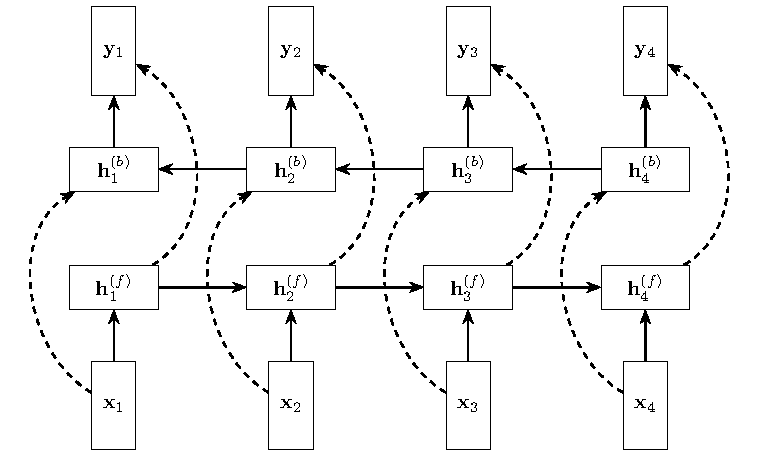
\includegraphics[width=0.7\textwidth]{tikz_image/rnn_bidirectional_architecture.pdf}
    \caption{Kiến trúc mạng hồi quy hai chiều}
    \label{figure:rnn-bidirectional-architecture}
\end{figure}

Mạng hồi quy hai chiều được chứng minh là xử lý tốt đối với các ứng dụng cần biết cả giá trị quá khứ lẫn tương lai. Nhưng đối với các ứng dụng không cần biết giá trị tương lai, mạng hồi quy hai chiều nhiều trường hợp vẫn cho ra độ chính xác cao hơn. Trong thực tế, các ứng dụng cần phải quan tâm cả quá khứ lẫn tương lai của dữ liệu có thể kể đến là nhận nhiện chữ viết tay (\textit{handwriting regconition}), ta dễ dự đoán nét chữ ở giữa hơn khi ta có thông tin về hai phía của nó. Mạng hồi quy hai chiều về cơ bản hoạt động như sau:
\begin{enumerate}
    \item Tính giá trị trạng thái ẩn tiến (\textit{forward hidden state}) $\mathbf h^{(f)}$ từ $t=0$ đến $t=T$ và tính giá trị trạng thái ẩn lùi (\textit{backward hidden state}) $\mathbf h^{(b)}$ từ $t=T$ đến $t=0$.
    \item Tính giá trị lớp đầu ra $\mathbf y_i=f(\mathbf h^{(f)},\mathbf h^{(b)})$.
    \item Tính giá trị đạo hàm hàm mất mát đối với mỗi lớp đầu ra.
    \item Tính giá trị đạo hàm hàm mất mát đối với từng trạng thái ẩn ($\mathbf h^{(f)},\mathbf h^{(b)}$) dùng thuật toán lan truyền ngược.
    \item Tính tổng các giá trị đạo hàm hàm mất mát tương ứng với các trọng số được chia sẻ $w$.
\end{enumerate}

\subsubsection{Mạng thần kinh hồi quy nhiều lớp (\textit{Multilayer Recurrent Network})}
Trong các ứng dụng thực tế, kiến trúc đa lớp mạng thần kinh được sử dụng để xây dựng các mô hình phức tạp hơn. Đối với mạng thần kinh truyền thống, lớp phía sau $\mathbf h_{k+1}$ sẽ được tính bằng lớp trước nó $\mathbf h_k$. Nhưng đối với mạng hồi quy đa lớp giá trị của một lớp $\mathbf h^{(k)}_t$ sẽ được tính bằng giá trị của lớp trước nó $\mathbf h^{(k-1)}_t$ và giá trị của lớp thời gian trước nó $\mathbf h^{(k)}_{t-1}$ (hình \ref{figure:rnn-multi-layer-architecture}).
\begin{figure}[htb]
    \centering
    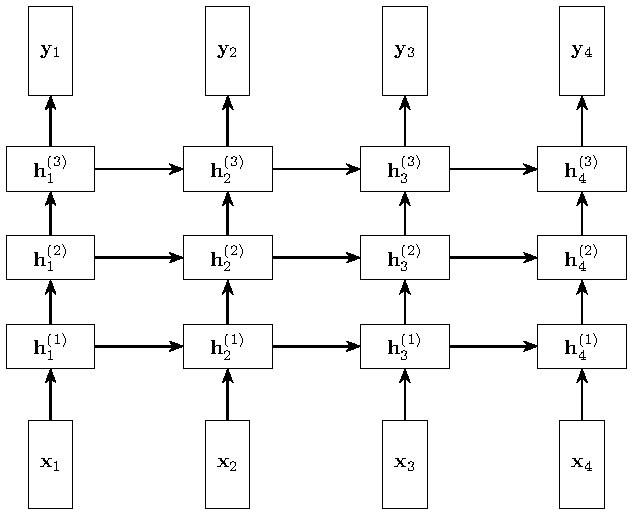
\includegraphics[width=0.6\textwidth]{tikz_image/rnn_multi_layer_architecture.pdf}
    \caption{Kiến trúc mạng hồi quy nhiều lớp}
    \label{figure:rnn-multi-layer-architecture}
\end{figure}

Đầu tiên, chúng ta viết lại phương trình tính lớp ẩn của mạng hồi quy một lớp, gọi $W^{(k)}_{t-1,t}$ là ma trận giữa lớp thời gian $t-1$ và $t$, cùng nằm trên lớp $k$, từ \ref{equation:rnn-h} ta có phương trình của lớp ẩn đầu tiên là
\begin{align}
    \mathbf h_t^{(1)}=\left[W_{xh},W^{(1)}_{t-1,t}\right]
    \begin{bmatrix}
        \mathbf x_t \\
        \mathbf h_{t-1}^{(1)}
    \end{bmatrix}
\end{align}
Đối với giá trị lớp ẩn đầu tiên, công thức sẽ khá giống bên trên. Gọi $W^{(k-1,k)}_{t}$ là ma trận trong cùng lớp thời gian $t$, giữa lớp $k-1$ và $k$. Gọi $W^{(k)}_{t}$ là ma trận biến đổi, ta có
\begin{align}
    \mathbf h_t^{(k)} & =\left[W^{(k-1,k)}_{t},W^{(k)}_{t-1,t}\right]
    \begin{bmatrix}
        \mathbf h_{t}^{(k-1)} \\
        \mathbf h_{t-1}^{(k)}
    \end{bmatrix}                                           \nonumber \\
                      & =W^{(k)}_{t}
    \begin{bmatrix}
        \mathbf h_{t}^{(k-1)} \\
        \mathbf h_{t-1}^{(k)}
    \end{bmatrix}\label{equation:rnn-multi-layer}
\end{align}

Thông thường số lượng lớp ẩn tầm hai hoặc ba là đủ. Đối với số lớp ẩn lớn rất dễ bị quá khớp, nên số lượng lớp ẩn tỉ lệ thuận với số lượng dữ liệu cho mô hình học.